\section{Introduction}
% \begin{figure}
%   \centering
%   \fbox{\rule[-.5cm]{0cm}{4cm} \rule[-.5cm]{4cm}{0cm}}
%   \caption{Sample figure caption.}
% \end{figure}
Online news portals such as BBC, CNN and Bing News have a huge number 
of readers daily. Many of them are anonymous or logged in as guests who typically don't read many stories in a single login session.
Given the limited interactions users engage with the portals, it is often 
hard for the systems to fully understand the user behavior, posing significant challenges to recommendation systems. 

Traditional news recommendation approaches rely on collaborative filtering and matrix factorization~\cite{cheng2016wide, guodeepfm2017, wang2018modeling, ge2020graph, hu2020graph, xie2020deep}
which requires the system to keep track of the user history and does not apply to anonymous 
visits or guest logins. 
Recent neural approaches for news recommendation mostly focus on encoding the text feature of articles with 
attention mechanism~\cite{wang2018dkn, zhu2019dan, wu_neural_2019-1, wu2019npa, wang2020fine, wu2020CPRS} 
when modeling user interest while paying little attention to the click behavior or 
the article-to-article transition. Thus they cannot take full advantage of the textual information 
when the interactions are sparse.

\begin{figure}[th]
    \centering
    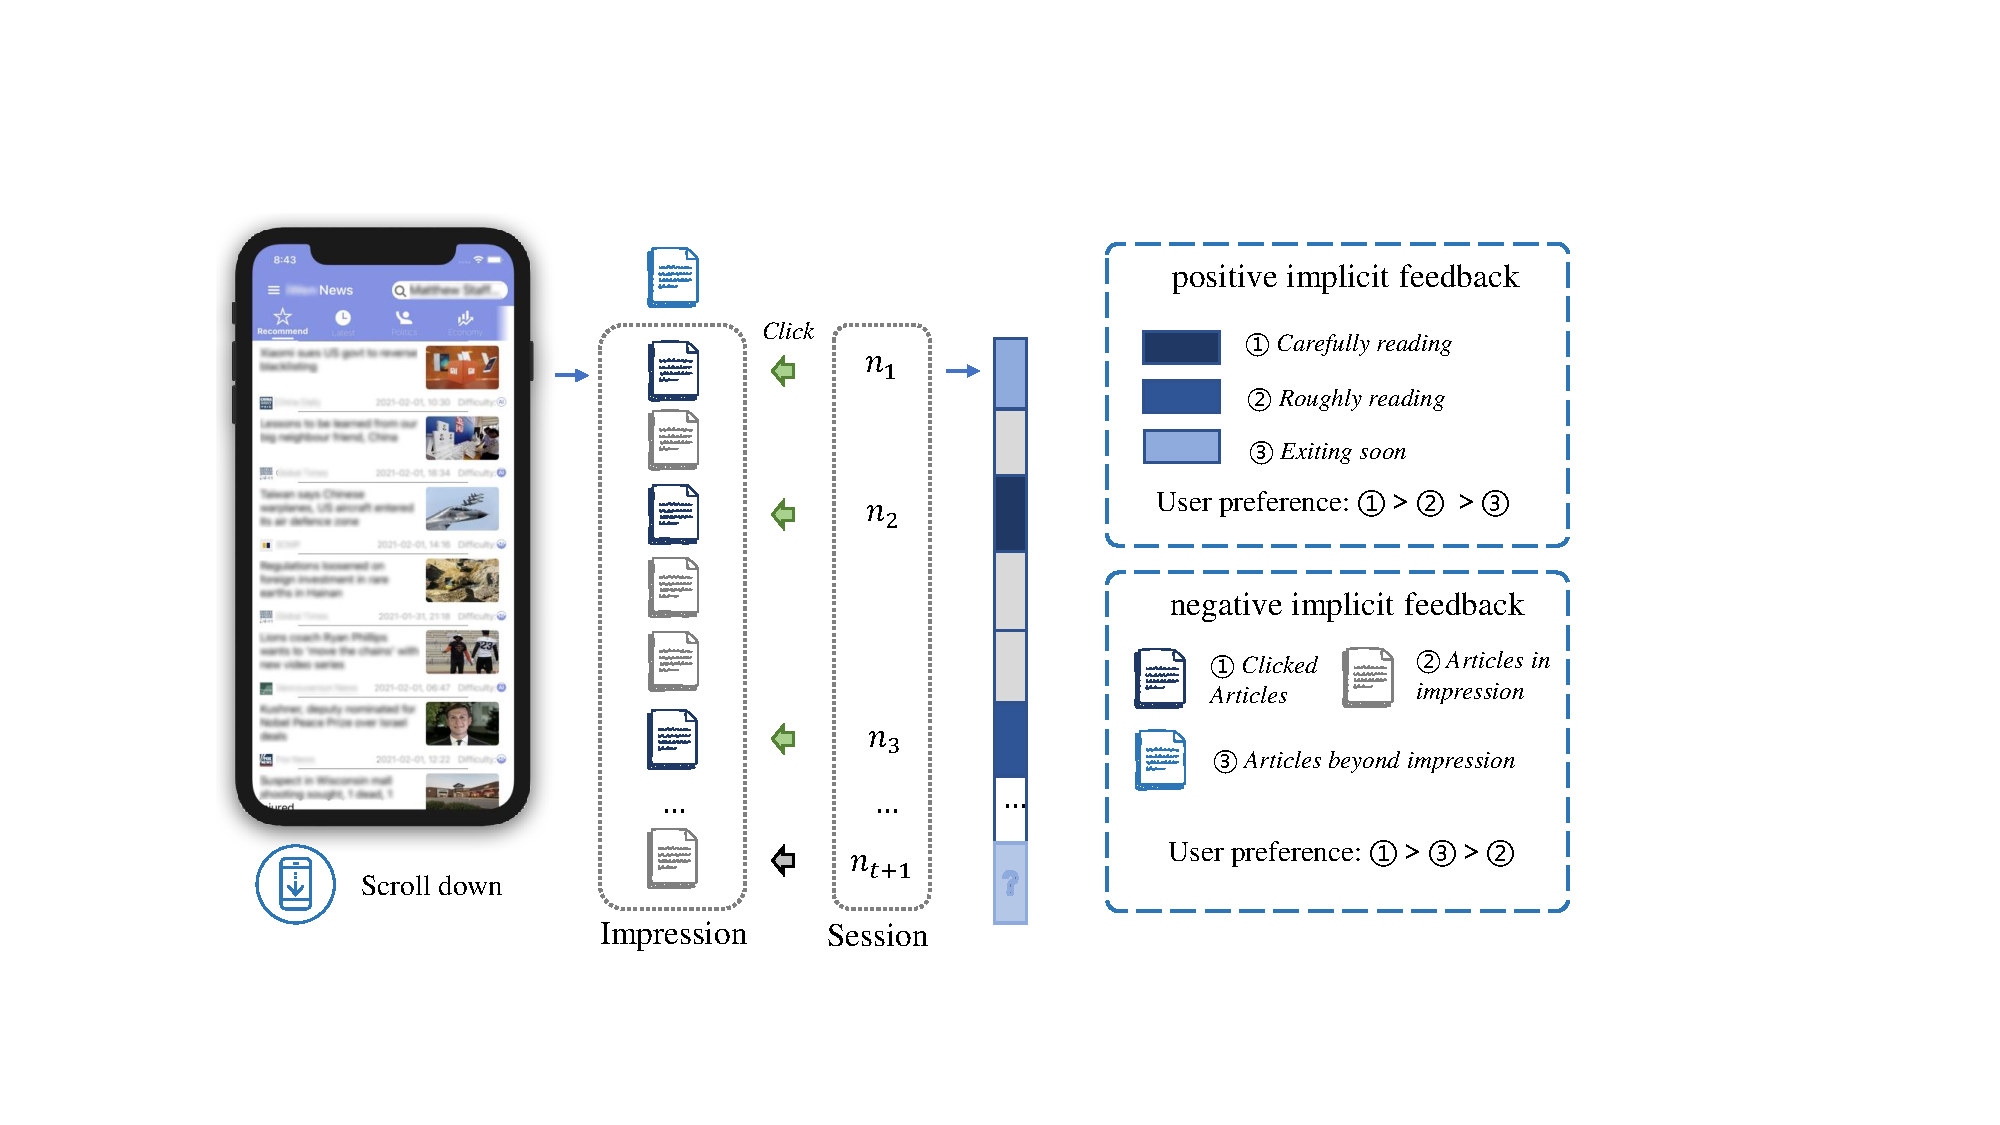
\includegraphics[width=\columnwidth]{fig/stream.pdf}
    \caption{A schematic of session-based news reading. 
    % A user may spend different amounts of time on different clicked articles, refering to different degrees of the implicit positive feedback, and the unclicked articles within/without impression list of the user also show different degrees of the implicit negative feedback. 
}
    \label{fig:session}
\end{figure}

On the other hand, session-based recommendation is widely used in the e-commerce or 
video streaming domain~\cite{ludewig2019performance, xu2019time, pan2020star},
where a \textit{session} is usually within a short time (e.g., 30 minutes) when the user is logged on. 
Thus, it's natural and realistic to formulate the news recommendation task for anonymous users as 
a session-based recommendation task to predict next item~\cite{epure_recommending_2017, sottocornola2018session, moreira_news_2018, symeonidis2020session}. However, they rarely consider the implicit feedback from user behaviors.

In this paper, we are interested in exploiting user actions besides the clicks themselves. We call them ``implicit feedback'', as
illustrated in \figref{fig:session}. 
Typical implicit feedback can be extracted from browsing the main page, 
reading an article, closing an article, backtracking~\cite{smadja_understanding_2019}, etc. We believe that modeling
this implicit feedback ``explicitly'' in the session-based recommendation systems
can help the recommender modeling the user's intention better. Here, we focus on answering 
these two questions:
\begin{enumerate}[label=(\roman*)]
    \item If a user clicks an article, does he/she really \textit{like} it? 
    \item If a user hasn't clicked an article, does he/she \textit{dislike} it?
\end{enumerate}

First, in traditional recommendation systems, ``clicks'' usually indicate a ``like'' or a
vote from the user, but it's a bit different for news reading. 
Users may be ``tricked'' into clicking an article~\cite{wang2020click} 
and once they realize that, they will quickly back out and switch to other articles. 
Thus the time a user spends on reading an article is a better, finer-grained gauge of the user's preference on the article~\cite{wu2020CPRS}, than just the click alone, which is only binary. We model this as the implicit positive feedback in this paper.
Second, among articles that the user didn't click on, the preference of the user varies too. Only the article exposed to the user while not being clicked 
conveys a stronger negative signal than those that never leave impressions to users~\cite{xie2020deep}.
Given that the user impression data is not always available, 
we \textit{infer} the impressions by assuming that articles are presented to the user roughly in the order of their publication time. 

Thus, in this paper, we formulate a session-based recommendation task to predict the next article 
for each session user from the candidate articles pool. Our main contributions are:
\begin{itemize} 
\item To the best of our knowledge, we are the first to leverage the positive/negative implicit feedback in anonymous session-based news recommendation. 
\item We design a method to leverage the 
implicit feedback in a simple way, which can be easily plugged into the basic attention network (\secref{sec:approach}). 
\item In our experiments, we conduct offline evaluations on three real-world datasets to show clear advantage
of our proposed method in terms of the trade-off between 
diversity and accuracy (\secref{sec:experiment}).
\end{itemize}
% This paper makes the following contributions: 
% \begin{itemize}
%     \item To the best of our knowledge, we are the first to leverage the positive/negative implicit feedback in anonymous session-based news recommendation;
%     \item Our method is very simple and can be easily plugged into other approaches.
%     \item Our comprehensive experiments on three real-world datasets show the promising performance and better trades off the dilemma between 
% diversity and accuracy. 
% \end{itemize}
